\section{Classification}

\subsection{A General Taxonomy of Sound}
% \begin{itemize}
%     \item Specialized models vs General model
%     \item Human perception as field of study
%     \item Gaver Taxonomy
%     \item Lewicki Added Context
%     \item Listening and hearing
% \end{itemize}

In the audio domain, it is often desirable to train specialized models instead
of investigating general models. For example, performant models have been
developed for tasks like speech recognition or music genre recognition with
specific features chosen for the task \cite{Campbell1997,
tzanetakis-musical-2002}. However, these approaches are not applicable to the
general case of audio recognition. Here, we propose using and extending upon an
ecological taxonomy of sound for our recognition model in an effort to make it
generalizable to diverse databases.

Studies of human perception have long been of interest to ecologists, one in
particular created a taxonomy of environmental sound based on physical
properties and human perception. He hypothesized that in general listening
tasks, humans rely on seemingly complex stimuli and not a combination of the
senses as was previously thought which if true means that an agent can determine
sources through audio alone. Gaver posits that sound provides information of
audio items interacting in the environment and that these kinds of interactions
can be separated into several classes and sub-classes. This hypothesis of
hearing breaks the problem of decoding what we hear into much more generalizable
pieces that an agent can be trained on \cite{Gaver1993}. Although Gaver's
taxonomy only creates a taxonomy for interacting materials in the environment,
other researchers have similarly studied perception of animal vocalizations and
music.

Lewicki's work aids in gaining a better understanding of how animal sounds will
fit into a general sound taxonomy \cite{lewicki-efficient-2002}. It is noted by
Lewicki that environmental sounds are structurally different from animal
vocalizations in that animal vocalizations are longer, harmonic, and have a
narrow bandwidth while environmental sounds are transient, non-harmonic, and are
broadband. He hypothesizes that this has intentionally evolved to allow for
easier discrimination from environmental sounds when communicating. However,
Lewicki finds that human speech is structurally different from normal animal
vocalizations in that it contains a mix of harmonic and non-harmonic structures.
As such, in the taxonomy, speech and animal vocalizations are two separate
branches.

Both Gaver and Lewicki make a distinction between how we listen normally and how
we listen to music. As such, even though speech and interacting elements
technically make up music, how we listen to and classify musical sounds is
different. Thus, music in the taxonomy makes up its own branch in the hierarchy
indicating that once the agent determines a sound is music, it will begin
listening to it differently.

\subsection{Hierarchy of Classifiers}

% \begin{itemize}
%     \item Hierarchical classification
%     \item Hierarchical vs Flat
%     \item Error propagation
%     \item Low level classifier overfitting
%     \item Probabilistic classifiers
%     \item Frame as formation of a probabilistic function with predicates (Blazeit)
%     \item Be sure to mention this is a task for specific tagging and retrieval (we do not wish to do the NLP lifting)
% \end{itemize}


\begin{figure}[h!]
    \centering
    \includegraphics[width=0.49\textwidth]{figures/ensemble-overview.png}
    \caption{An overview of the proposed ensemble classifier.}
    \label{fig:classifier-hierarchy}
\end{figure}

Most classification tasks are what are called \textbf{flat classification}
meaning there is no hierarchy between the categories or if there is, it is
ignored. Our classification model instead uses the above taxonomy as a guide for \textbf{hierarchical classification} with a top-down approach. In a hierarchical model, multiple classifiers are trained on the same data. Unlike other ensemble methods though, this model trains each classifier with different goals \cite{chou-hierarchical-2003}. Here, we train a classifier per level of the tree. In evaluation, the algorithm follows a classification path, choosing a direction as each level is evaluated. This approach increases overall performance by breaking the classification task into smaller and less complex problems. Additionally, this approach allows us to throw out clearly irrelevant documents early, improving query runtime.

\subsubsection{Risks}
Error propagation is a major issue in this approach and if not managed can ruin the approach outright. Each classifier has some classification error inherent to it and as such a high error on higher level classifiers can seriously impede the efficacy of the system as a whole. We address this through use of probabilistic classifiers, enabling a measure of certainty, and how retrieval of documents is carried out.

Another consideration when working with a hierarchical classifier is whether the lowest level classes have enough examples to train a general model. If too few examples of a low-level class are in the database, the classifiers will begin to overfit. To mitigate this issue, another threshold policy is introduced. This time, the threshold is the minimum number of examples required to allow a classifier to be trained on a certain class. This results in instances of the model trained on a smaller database being less precise in their retrieval.

\subsection{Classification Methods}

\begin{table}[t]
    \centering
    \begin{tabular}{ccc}
         & 250   & 2000  \\ \hline
    DNN  & 0.174 & 0.191 \\
    HDNN & 0.246 & 0.130
    \end{tabular}
    \caption{Classification results of a hierarchical DNN and a standard DNN trained on all 50 classes.}
    \label{tab:classifier}
\end{table}

\begin{itemize}
    % \item Argue non-uniform classifier use
    \item Filtering Classifiers
    \item Deciding Classifiers
\end{itemize}
Specific contexts of audio classification have long been an area of interest and thus certain audio sub-domains have been extensively studied for optimal classification techniques. It is unlikely that in human perception all different listening tasks are accomplished through the same process. Instead there are likely specialized systems that have evolved to best handle specific classification tasks. Using this intuition and the ability to do so through hierarchical classification, we pick and choose classifiers and representations that work best for each sub-domain. As this is a tree hierarchy, we have branch and leaf nodes that are comprised of their own classifier. Here, we term them \textit{Filtering} and \textit{Deciding} classifiers.

\subsubsection{Filtering Classifiers}

\begin{table}[h]
    \begin{tabular}{c|cc}
        Classifier & Training & Prediction \\ \hline
        SVM & $O(n^2p+n^3$ & $O(n_{sv}p)$ \\
        KNN & - & $O(np)$ \\
        RFC & $O(n^2\sqrt{p}n_{trees})$ & $O(pn_{trees})$
    \end{tabular}
\caption{Filtering classifiers and their properties.}
\label{tab:filt-class}
\end{table}

Filtering classifiers are the branch nodes of the hierarchy tree. They have this term as their main purpose is to filter the data and throw out unrelated documents such that lower filter and deciding classifiers can execute more quickly. In our experiments, it was found to be desirable for these classifiers to be both lightweight and have uncertainty associated with it. As such, probabilistic classifiers are used in the filtering classifiers. 

Probabilistic classifiers are key to mitigating the issue of error propagation in the hierarchical model. While standard classifiers emulate a function of the form $y=f(x)$ with a single result \textit{y} for each input \textit{y}, a probabilistic classifier instead emulates conditional distributions of the form $P(y|x)$. We are able to use the resulting probabilities given by a classifier to determine its confidence in the prediction made. We use this confidence to allow normally misclassified results to still be considered in later steps. This is done by introducing a threshold $\gamma$ that must be reached to proceed. If the threshold is too low, we lose the performance efficacy of the hierarchical structure. On the other hand, if the threshold is too high then false negatives will ensure some documents with harder to classify instances of a class will never be retrieved.

In this implementation, the following lightweight and probabilistic classifiers were experimented with:
\\
\\
\textbf{Support Vector Machines} are a supervised learning model used for classification that partitions the data by finding the most optimal linear hyper-plane that separates all dimensions of the feature set optimally. Although SVMs inherently separate the data by some linear relationship (decision boundary), non-linear classification can be done by the kernel trick. The kernel trick is the method of mapping the inputs into different feature spaces in which the data is linearly separable. To allow for probabilistic estimation, the SVM is computed with soft-margins. The soft-margins provide a decision boundary with in-built uncertainty through a gradient of certainty that becomes greater as samples are picked further from the boundary. The boundary is calculated by minimizing the the hinge loss function over all samples. This is calculated by

\begin{equation}
    \Big[ \frac{1}{n}\sum^n_{i=1}\max(0,1-y_i(\vec{\omega} \cdot \vec{x_i} - b))\Big] + \lambda ||\vec{\omega}||^2
\end{equation}
\\
where $\omega$ is the normal vector to the hyper-plane, $y_i$ is the target, $\vec{x_i}$ is the features at i, and $\lambda$ determines the margin size and whether $\vec{x_i}$ is on the correct side of the decision boundary. For small values of $\lambda$, the soft-margin SVM will perform similarly to the hard-margin.
\\
\\
\textbf{K-Nearest Neighbors} is a classification method that uses the plurality vote of its neighbor samples by some heuristic of distance to determine its belonging to a class. KNN is known as a \textit{lazy learning} method, meaning the classifier defers its computation until classification evaluation. As such, all points are retained in the model. Any custom heuristic for distance can be used but the most common is Euclidean distance or Manhattan Distance. One of the more challenging parts of this classification approach is the tuning of the neighbor number hyper-parameter as at k=1 the class is determined by the first closest neighbor and at k=n the class is whatever the most numerous of the classes is present. To use this classifier in a probabilistic case, the number of matching neighbors and the distances can be used for determination. Probability is computed such that the radial area surrounding the k neighbors creates a probability distribution. \cite{cheng-evaluating-2009}
\\
\\
\textbf{Random Forests} are a supervised ensemble classification learning method. This method uses a collection of decision tree classifiers and at evaluation time provides the mode of the classification prediction. This method attempts to correct for decision trees tendency to overfit the training set. Specifically, deep trees more often tend to overfit, have low bias, and very high variance. Thus, by training many trees on multiple parts of the data, it is expected that variance will be reduced with only a small increase in bias. To train a random forest, the bagging algorithm is employed. This algorithm takes a training set and selects a random sample with replacement to fit a tree to. The bagging approach decreases the model variance, which as mentioned before is a problem in decision trees, and only slightly increases the bias. Evaluation of the model is straightforward as it is either an average of the data in the regression case or is majority vote in classification. To provide probability to the random forest classifier, the choice between two paths is treated as a probability density function (pdf) and both branches are evaluated if it meets some criterion for acceptable probability bounds \cite{. This approach 
\\
% \subsubsection{Annotation Normalization} Annotation normalization is carried
% out on subsets of both the ESC-50 and AudioSet database. Performance is
% measured in terms of execution time, efficiency, and overall annotation
% reduction. The normalization performance is measured against human performance
% and Hsu's normalization results \cite{Hsu2008}. As ESC-50 already has its
% annotations manually normalized, the normalization experiments demonstrate if
% the techniques go too far and overgeneralize. Additionally, it provides a
% clean test-bed for hypernyms to be evaluated. For hypernym sets, we hope to
% have sets that as much as possible attempt to distribute the database across
% them. AudioSet presents a much greater challenge for the low level
% normalization task. These experiments give insight into how the technique
% works at scale and what bottlenecks exist.

\subsubsection{Deciding Classifiers}
\begin{table}[h]
    \begin{tabular}{c|cc}
        Classifier & Training & Prediction \\ \hline
        DNN & $O(n^4)$ & $O(n^5)$ \\
        RNN & $O(n^4)$ & $O(n^5)$ \\
        GMM & $NP$ & $a$
    \end{tabular}
    \caption{Decision classifiers and their properties.}
    \label{tab:dec-class}
\end{table}
paragraph
\\
\textbf{Deep Neural Networks}
\\
\textbf{Long-Short Term Neural Networks}
\\
\textbf{Gaussian Mixture Model}
\\

\begin{figure}
    \centering
    \includegraphics[width=0.45\textwidth]{example-image-a}
    \caption{Plot of feature reduced samples from music, animal, speech, and environmental sounds}
    \label{fig:top-dist}
\end{figure}

